%File: formatting-instructions-latex-2024.tex
%release 2024.0
\documentclass[letterpaper]{article} % DO NOT CHANGE THIS
\usepackage{aaai24}  % DO NOT CHANGE THIS
\usepackage{times}  % DO NOT CHANGE THIS
\usepackage{helvet}  % DO NOT CHANGE THIS
\usepackage{courier}  % DO NOT CHANGE THIS
\usepackage[hyphens]{url}  % DO NOT CHANGE THIS
\usepackage{graphicx} % DO NOT CHANGE THIS
\urlstyle{rm} % DO NOT CHANGE THIS
\def\UrlFont{\rm}  % DO NOT CHANGE THIS
\usepackage{natbib}  % DO NOT CHANGE THIS AND DO NOT ADD ANY OPTIONS TO IT
\usepackage{caption} % DO NOT CHANGE THIS AND DO NOT ADD ANY OPTIONS TO IT
\frenchspacing  % DO NOT CHANGE THIS
\setlength{\pdfpagewidth}{8.5in}  % DO NOT CHANGE THIS
\setlength{\pdfpageheight}{11in}  % DO NOT CHANGE THIS
%
% These are recommended to typeset algorithms but not required. See the subsubsection on algorithms. Remove them if you don't have algorithms in your paper.
\usepackage{algorithm}
\usepackage{algorithmic}

%
% These are are recommended to typeset listings but not required. See the subsubsection on listing. Remove this block if you don't have listings in your paper.
\usepackage{newfloat}
\usepackage{listings}
\DeclareCaptionStyle{ruled}{labelfont=normalfont,labelsep=colon,strut=off} % DO NOT CHANGE THIS
\lstset{%
	basicstyle={\footnotesize\ttfamily},% footnotesize acceptable for monospace
	numbers=left,numberstyle=\footnotesize,xleftmargin=2em,% show line numbers, remove this entire line if you don't want the numbers.
	aboveskip=0pt,belowskip=0pt,%
	showstringspaces=false,tabsize=2,breaklines=true}
\floatstyle{ruled}
\newfloat{listing}{tb}{lst}{}
\floatname{listing}{Listing}
%
% Keep the \pdfinfo as shown here. There's no need
% for you to add the /Title and /Author tags.
\pdfinfo{
/TemplateVersion (2024.1)
}

% DISALLOWED PACKAGES
% \usepackage{authblk} -- This package is specifically forbidden
% \usepackage{balance} -- This package is specifically forbidden
% \usepackage{color (if used in text)
% \usepackage{CJK} -- This package is specifically forbidden
% \usepackage{float} -- This package is specifically forbidden
% \usepackage{flushend} -- This package is specifically forbidden
% \usepackage{fontenc} -- This package is specifically forbidden
% \usepackage{fullpage} -- This package is specifically forbidden
% \usepackage{geometry} -- This package is specifically forbidden
% \usepackage{grffile} -- This package is specifically forbidden
% \usepackage{hyperref} -- This package is specifically forbidden
% \usepackage{navigator} -- This package is specifically forbidden
% (or any other package that embeds links such as navigator or hyperref)
% \indentfirst} -- This package is specifically forbidden
% \layout} -- This package is specifically forbidden
% \multicol} -- This package is specifically forbidden
% \nameref} -- This package is specifically forbidden
% \usepackage{savetrees} -- This package is specifically forbidden
% \usepackage{setspace} -- This package is specifically forbidden
% \usepackage{stfloats} -- This package is specifically forbidden
% \usepackage{tabu} -- This package is specifically forbidden
% \usepackage{titlesec} -- This package is specifically forbidden
% \usepackage{tocbibind} -- This package is specifically forbidden
% \usepackage{ulem} -- This package is specifically forbidden
% \usepackage{wrapfig} -- This package is specifically forbidden
% DISALLOWED COMMANDS
% \nocopyright -- Your paper will not be published if you use this command
% \addtolength -- This command may not be used
% \balance -- This command may not be used
% \baselinestretch -- Your paper will not be published if you use this command
% \clearpage -- No page breaks of any kind may be used for the final version of your paper
% \columnsep -- This command may not be used
% \newpage -- No page breaks of any kind may be used for the final version of your paper
% \pagebreak -- No page breaks of any kind may be used for the final version of your paperr
% \pagestyle -- This command may not be used
% \tiny -- This is not an acceptable font size.
% \vspace{- -- No negative value may be used in proximity of a caption, figure, table, section, subsection, subsubsection, or reference
% \vskip{- -- No negative value may be used to alter spacing above or below a caption, figure, table, section, subsection, subsubsection, or reference

\setcounter{secnumdepth}{0} %May be changed to 1 or 2 if section numbers are desired.

% The file aaai24.sty is the style file for AAAI Press
% proceedings, working notes, and technical reports.
%

% Title

% Your title must be in mixed case, not sentence case.
% That means all verbs (including short verbs like be, is, using,and go),
% nouns, adverbs, adjectives should be capitalized, including both words in hyphenated terms, while
% articles, conjunctions, and prepositions are lower case unless they
% directly follow a colon or long dash
\title{\textbf{COMP 370 Final Project - Movie Release}}
\author{
    \textbf{Written by} \\ 
    Owen Le Sann (261102284), Lucas Loghin (261054119), Giannino Lombardi (261051827) \\
    \vspace{5pt}
    {\small McGill School of Computer Science \\ 
    owen.lesann@mail.mcgill.ca, lucas.loghin@mail.mcgill.ca,
    giannino.lombardi@mail.mcgill.ca}
}



% REMOVE THIS: bibentry
% This is only needed to show inline citations in the guidelines document. You should not need it and can safely delete it.
\usepackage{bibentry}
% END REMOVE bibentry

\begin{document}

\maketitle

\section{Abstract}

This project aims to assess the reception and public opinion of Francis Ford Coppola’s latest film, \textit{Megalopolis}. We analyze the film’s media coverage and critical reception, comparing its performance to other movies released within the four weeks before and after its debut. Through rigorous open-coding, we developed a typology to identify the particular topics associated with \textit{Megalopolis} that have garnered the most attention. By examining these patterns, we provide Lionsgate Films with valuable insights into the impact of its latest production.

\section{Introduction}

Journalistic film criticism provides an essential platform for the public to voice their opinions about a film, comprising a large share of free marketing for film distributors. On average, 53\% of people say they are exposed to news media criticisms "very" or "quite often" \cite{robertson2023}. Moreover, it has been shown that the tone of these criticisms directly correlates to a film's box office earnings over eight-week periods \cite{basuroy2003}. These studies may incline film distributors to seek a holistic view of the reception and visibility of their films relative to those released in a similar time frame by competing distributors.
\\
\\
\textit{Megalopolis}, anticipated as Francis Ford Coppola's magnum opus, is a film whose performance is particularly subject to public criticism. Will \textit{Megalopolis} be eternalized as a masterpiece and watched for years to come, or will it be a flop tainting the reputation of Mr. Coppola and the profits of the company distributing it? Lionsgate Films, the film's distributor, has approached us regarding just that. Notably, they are interested in determining what aspects of the movies have gained the most attention. In addition, they are also interested in determining what proportion of online journalistic criticisms talk about \textit{Megalopolis} relative to other movies released within a four-week period of the September 27, 2024, release date of \textit{Megalopolis}.
\\
\\
To better define our data and the results derived from it, below we expand on some important terminology:

\begin{itemize}
    \item An online journalistic criticism is an analysis and evaluation of a film written by a professional film critic and published as an online news article. These criticisms are interpreted as more subjective expressions of the film's content, style, and production values. In our study, we aim to objectively categorize the foci of our articles into eight well-defined categories detailed in our annotation methodology. In this study, we assume that every collected article mentioning one of the five selected films in the article's title is an online journalistic criticism.
    
    \item An eight-week period defined in this study is a time interval containing eight weeks before and eight weeks after the date of interest inclusive. Likewise, a four-week period is an interval containing four weeks before and four weeks after the date of interest.

\end{itemize}
Following the analysis of more than 500 news articles, we arrived at several exciting findings:
\begin{enumerate}
    \item The overall coverage of \textit{Megalopolis} received a balanced amount of media coverage, standing alongside other big movies.
    
    \item Coppola's reputation as a director heavily influenced the prevalent topics of discussion regarding \textit{Megalopolis}.
    
    \item Post-release coverage for \textit{Megalopolis} saw a significant rise compared to other movies.

\end{enumerate}

Note that Joker 2 refers to \textit{Joker: Folie à Deux} and Venom 3 refers to \textit{Venom: The Last Dance}. 

\section{Data}

Our cleaned and annotated dataset comprised 510 online journalistic criticism records, each with seven fields:

\begin{enumerate}
    \item \textbf{Title}: The title of the journalistic news criticism.
    
    \item \textbf{Author}: The author of the journalistic news criticism.
    
    \item \textbf{Published Date}: The date published in ISO 8601 format.
    
    \item \textbf{Link}: The link to the source of the online journalistic criticism.
    
    \item \textbf{Summary}: A summary of the article's written text.
    
    \item \textbf{Movie}: The movie from our list of movies that the online journalistic article discusses.
    
    \item \textbf{Article Focus}: The focus on the article from our well-defined list of focus categories.
\end{enumerate}

Building this dataset took many careful considerations, the first determining which films we wanted to compare \textit{Megalopolis} against. We essayed to select a list of films that best represented \textit{Megalopolis}' competition. For us, a film that competes with \textit{Megalopolis} is one debuting in a similar region to a similar demographic with a competitive production budget and is marketing against and debuting in theaters around the same time as \textit{Megalopolis}s. To satisfy this definition, we selected films released within a four-week period of \textit{Megalopolis}, which were North American films with a production budget greater than ten million USD. These films, including \textit{Megalopolis} and accompanied by their U.S. theatrical debut and production budget in USD, are:

\begin{enumerate}
    \item \textbf{Megalopolis}
    \begin{itemize}
        \item Debuted on September 27, 2024.
        \item Production budget of \$120 million.
    \end{itemize}
    
    \item \textbf{Venom: The Last Dance}
    \begin{itemize}
        \item Debuted on October 25, 2024.
        \item Production budget of \$120 million.
    \end{itemize}
    
    \item \textbf{The Wild Robot}
    \begin{itemize}
        \item Debuted on September 27, 2024.
        \item Production budget of \$78 million.
    \end{itemize}
    
    \item \textbf{The Substance}
    \begin{itemize}
        \item Debuted on September 20, 2024.
        \item Production budget of \$17.5 million.
    \end{itemize}
    
    \item \textbf{Joker: Folie à Deux}
    \begin{itemize}
        \item Debuted on October 4, 2024.
        \item Production budget of \$200 million.
    \end{itemize}
\end{enumerate}

Having our movies in order, we collected our film data. To better perform our annotation and analysis, we ensured that we had more than 500 records and that each record in our online journalistic criticism had the following features:

\begin{itemize}
    \item It was published within an eight-week period of the U.S. theatrical debut of \textit{Megalopolis}.
    
    \item Most of its summary, 95\% of all words, are written in English.
    
    \item It writes about one of our five movies with 95\% accuracy.
    
    \item It is unbiased towards or against the coverage volume of our selected movies.
\end{itemize}

\section{Methods}

\subsection{Initial Attempts}

A lot of trial and error led to a dataset that exhibited all the features detailed above. At the genesis of this project, we had initially intended to use NewsAPI’s API to source our unsampled and unannotated online journalistic criticism records. However, we soon realized that this API needed to improve its querying capabilities. For instance, the API:

\begin{enumerate}
    \item \textbf{Could not query articles published within an eight-week period of the U.S.} theatrical debut of \textit{Megalopolis}. The free tier lookback period for the API is 30 days from the time of the API call, which, for us, was 30 days preceding November 25, 2024. In other words, the earliest articles available to us through the NewsAPI were those published on or after October 26, 2024. This was a problem, as we wanted to study articles published within an eight-week period of \textit{Megalopolis}' September 27, 2024, theatrical debut, meaning that we would need to access articles published on or after August 2, 2024—more than two months exceeding NewsAPI's capabilities.
    
    \item \textbf{Could only query a limited number of articles per day.} The free tier API allows a maximum query of 100 online journalistic criticisms per day. Because we wanted to uniformly random sample our 500 records and because we wanted this sample to comprise at most 15\% of the population to minimize sampling bias, we needed at least 3334 unique journalistic news criticisms for this study. This meant that it would take a minimum of 50 days to source our online journalistic criticisms, which greatly exceeded our personal time frame for the data collection in this study, which was 14 days.
\end{enumerate}

With these blaring issues, we needed to switch to a new tool: NewsCatcher API. The NewsCatcher API initially granted us:

\begin{itemize}
    \item 2000 API calls
    \item One call per second
    \item 1000 articles per call
    \item Two-week lookback
    \item An exact querying algorithm
\end{itemize}

Moreover, after contacting the team, they kindly extended our lookback period from 14 days to 180 days free of charge. This API enabled us to query all 5000 online journalistic criticisms accurately, focusing exclusively on our five films in our eight-week period of \textit{Megalopolis}' theatrical debut in just five seconds.

\subsection{Data Collection and Filtering}

With this powerful API in our toolkit, we were ready to collect our data. Our data collection followed a two-step process. Firstly, we collected 5000 English-language films whose titles included one or more of our five movies and who were in an eight-week period of \textit{Megalopolis}' theatrical debut, which was the interval from August 2, 2024, to November 22, 2024, inclusive. After collecting the initial records, we ran a separate script to filter out duplicates in the titles, which we found accounted for almost all the duplicate records, uniformly randomly sampling 600 records from this filtered dataset. Our initial filtering dropped our record count from 5000 to 4886 entries, from which we sampled 600 records, of which another 43 duplicate entries were manually removed during our open coding—leaving us with 557 unique records, 510 of which were annotated. We believe that by considering movies within a four-week period of \textit{Megalopolis}' theatrical debut and by uniformly randomly sampling films comprising less than 15\% of our record population, we have not only minimized the bias associated with centering our eight-week period on the theatrical debut of \textit{Megalopolis} but also minimized any bias that would originate from caching by NewsCatcher's querying algorithms or responses to our API requests.



\subsection{Typology Building}

As previously outlined, one of the main objectives of our study was to determine the topics that particularly caught moviegoers’ attention when seeing \textit{Megalopolis} in theatres. With this in mind, a typology was necessary. To create this categorization system, we began by open-coding the first 200 entries of our data set. This resulted in the identification of five preliminary categories: Gross Earnings, Plot/Cast, Critical Reception, Anticipation/Marketing, and Merchandising. Upon further discussion, these categories were expanded in order to better capture the nuances within the data. 

Plot/Cast was split into two separate categories: Plot/Themes and Cast and Crew/Characters. This allowed us to differentiate between the movie’s narrative elements and the individuals involved at all levels of its creation. Most notably, this stratification helped account for articles pertaining to a given crew member’s life outside of the context of the film. 

Public Opinion/Media Coverage was created as a branch of the Critical Reception category. Above all else, this allowed us to separate the opinions of industry experts. These individuals’ opinions carry a certain level of authority in comparison to social media posts or aggregated scores, which often reflect the perspectives of less qualified individuals. 

Anticipation/Marketing was split into two distinct categories. The Merchandising category was subsequently merged into the newly-created Marketing category. The goal of this decision was to differentiate between the organic buzz and anticipation surrounding a movie’s upcoming release and the deliberate efforts by entertainment companies to market its latest production. 

Finally, we recognized the need for an Unrelated category. It became abundantly clear its absence greatly hindered the comprehensiveness of our typology. Certain article entries, particularly those related to Venom, contained information (i.e. venomous animals, VENOM stock updates, etc.) that was entirely irrelevant to our study.

The resulting typology contained eight distinct categories: Gross Earnings, Public Opinion/Media Coverage, Critical Reception, Cast and Crew/Characters, Plot/Themes, Anticipation, Marketing, and Unrelated. The open-coding process equipped us with a clearly-defined approach for the remainder of the annotation. The categorization of most entries was straightforward and simply involved scanning the article's title. In complex cases, we viewed the article’s summary in order to make a more informed decision. 

\subsection{Analysis}

Once the annotated data was ready, we calculated the term frequency-inverse document frequency (TF-IDF) for our topics. We focused on the text from the Summary column in our data and split the articles according to their corresponding annotations. We first preprocessed the data in four steps. First, we ensured that case sensitivity wouldn't affect our results so we used the lower() method on the data. Then we used re.sub to removed all punctuations and special symbols, followed by tokenization of the data using split(). Lastly, we used the NLTK stopword file and added the movie titles to to filter the words, because otherwise we'd just have the movie titles as the top words for most of the categories. With the preprocessed data ready, all that remained was to compute the TF-IDF scores for each word and computed the top 10 words for each category. 

\section{Results}
\subsection{Typology Definitions}

After conducting open-coding on the first 200 articles in our data set, the following categorization system was established:

\begin{itemize}
    \item \textbf{Gross Earnings:}  
    Articles that discuss the financial success of the film. Box office revenue, cumulative gross, and performance across international markets are typical talking points in these articles.  
    Positive example: “Chris Sanders’ The Wild Robot debuts at \#1.” This falls under the Gross Earnings category as it assesses how much box office revenue the movie has accumulated in comparison to others released within the same time frame.  
    Negative example: “The Wild Robot reviews: a "stunning," "magnificent" film with "remarkably subtle" Lupita Nyong’o performance.” This article focuses on the public’s appreciation for the film rather than its financial success.  
    Edge case: “Francis Ford Coppola’s \$120m epic Megalopolis leaves audiences divided on Rotten Tomatoes.” While this article title mentions the budget for Megalopolis, the main takeaway is the public’s negative outlook on the production. Therefore, it does not fall into the Gross Earnings category.  

    \item \textbf{Public Opinion/Media Coverage:}  
    Articles that assess how a movie has been received by the general public. These articles often include social media conversations, audience ratings, and performances on aggregated scores like Rotten Tomatoes.  
    Positive example: “Demi Moore’s gory horror film The Substance qualifies as comedy at Golden Globes, and fans are divided.” This article falls into Public Opinion/Media Coverage because it references social media discourse about the film’s classification as a comedy.  
    Negative example: “Venom 3 finally introducing Spider-Man in Sony’s Marvel Universe just got a lot more likely.” This article mostly entails speculation/predictions in the days leading up to the release of the film and is not a direct reaction to its content.  
    Edge case: “Megalopolis box office finally passes its first global milestone (but it’s still a disastrous release).” This article hints at the negative public reception of Megalopolis, but its primary focus is the financial aspect of the film’s release.  

    \item \textbf{Critical Reception:}  
    Articles that contain film evaluations from industry professionals, critics, and journalists. Movie reviews and detailed critiques frequently fall into this category.  
    Positive example: “Movie review: The Wild Robot, the best animated film of the year.” This article is an industry expert’s review of The Wild Robot, during which the critic’s favorite and least favorite aspects are outlined.  
    Negative example: “Optimism grows for The Wild Robot sequel as film exceeds expectations.” This article notes the overall optimism surrounding the film’s release but does not contain a detailed critique from a well-respected individual.  
    Edge case: “Joker 2 gets the most surprising fan.” This article explains that, despite a negative public sentiment for Joker 2, Quentin Tarantino enjoyed the film. Given Tarantino’s standing in the film industry and the depth of his analysis in this article, it qualifies as a Critical Reception entry.  

    \item \textbf{Cast and Crew/Characters:}  
    Articles that showcase the diverse individuals involved in the creation of a film, along with the characters portrayed by its actors. This category includes assessments of individual performances, as well as coverage of appearances in interviews, red-carpet events, and other promotional activities.  
    Positive example: “Megalopolis extra allegedly kissed by Francis Ford Coppola in set video speaks out: 'I was in shock.'” This article describes an off-camera incident between two members of the movie’s crew and therefore falls into this category.  
    Negative example: “Francis Ford Coppola’s Megalopolis flops at the box office as The Wild Robot takes the top spot.” This article mentions the movie’s director but focuses on its box office performance above all else.  
    Edge case: “The Wild Robot, starring Nyong’o and Pedro Pascal, receives release date in India.” While this article mentions the movie’s primary actors, it does not go into depth about their personalities and/or respective roles. As a result, it does not qualify for Cast and Crew/Characters.  

    \item \textbf{Plot/Themes:}  
    Articles that offer an in-depth analysis of a movie’s plot and the underlying themes it explores. These pieces often highlight the film’s core messages and examine how effectively they resonate with audiences.  
    Positive example: “The set design of The Substance means more than you think.” This article explains how The Substance effectively uses set design to underscore the metaphors of beauty standards and confidence with one’s body.  
    Negative example: “The Wild Robot boasts beautiful animation, great voice acting by Lupita Nyong’o, and a soaring score.” This article briefly mentions the film's contents but focuses on the positive feedback it’s been getting from the general public.  
    Edge case: “'For my beloved': who Megalopolis is dedicated to.” While the movie’s plot is mentioned when describing who Megalopolis was dedicated to, the article’s emphasis is on the relationship between Francis Ford Coppola and his wife. It therefore falls under Cast and Crew/Characters instead.  

    \item \textbf{Anticipation:}  
    Articles that are published in the weeks leading up to a film’s debut that convey excitement and build anticipation. Examples include trailer reactions, predictions, and updates about the movie’s release.  
    Positive example: “The Venom 3 trailer teased a secret symbiote power only Marvel fans caught.” This article reacts to the release of Venom 3’s trailer and speculates about a new power being introduced in the movie.  
    Negative example: “Wait, is [spoiler] really dead after Venom: The Last Dance?!” This article speculates about an open-ended topic that arose after the release of Venom 3.  
    Edge case: “Joker 2 global box office continues spiraling ahead of digital debut.” This article was released ahead of the digital debut, but the movie had already been released in theaters. Therefore, it does not qualify for Anticipation.  

    \item \textbf{Marketing:}  
    Articles that cover products and events that are meant to advertise a movie. Examples include merchandise, film festivals, and themed events.  
    Positive example: “Shop Marvel must-haves: the best official Venom merch.” This article is promoting official products associated with Marvel’s latest Venom release.  
    Negative example: “Megalopolis’ first full trailer insists it will stand the test of time.” This article is, above all else, a reaction to a movie trailer and thus falls under the Anticipation category instead.  
    Edge case: “The Wild Robot wins Scad Savannah film festival audience award.” While this article refers to a film festival, it is more of a reflection on the general public’s appreciation for The Wild Robot. Therefore, it falls into the Public Opinion/Media Coverage category.  

    \item \textbf{Unrelated:}  
    Articles that contain the movie’s title but do not discuss the movie itself.  
    Positive example: “Venomous blue sea dragons wash ashore in Outer Banks.” This article mentions Venom in the context of dangerous venomous animals rather than the Marvel series.  
    Negative example: “'What did they do to Tom Hardy?': Tom Hardy’s transformation in Venom movies sparks concern, but was it intentional?” This article keys in on one of Venom’s most important characters.  
    Edge case: “4 words just permanently transformed Spider-Man \& Venom’s rivalry.” While this article does not necessarily focus on Venom 3, it goes into depth about its main character and therefore qualifies for Cast and Crew/Characters.  
\end{itemize}

\subsection{Analysis Results}

The first analysis quantified the total number of articles per movie. Then, we set a specific 4 week time frame, 2 weeks before and after each movie release date to get an  insight on how coverage evolved around the release of each movie. Lastly, with the now 510 articles annotated, we computed the article topic distribution for each movie and compared them. 

\subsection{TF-IDF Results}

The top 10 words, i.e. most representative words, for each topic was computed using TF-IDF analysis. The results have been submitted as a separate file and will be referenced in the upcoming section.


\begin{figure}
    \centering
    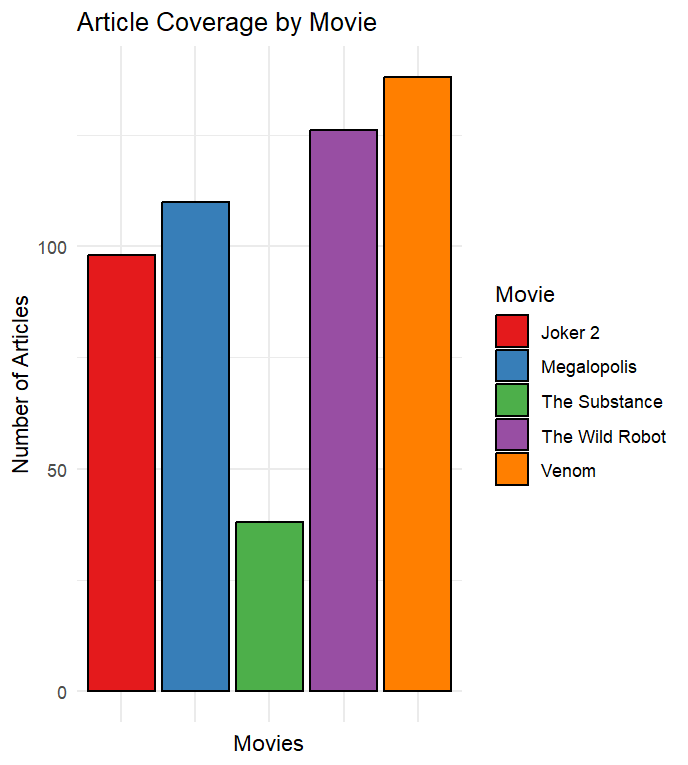
\includegraphics[width=0.4\textwidth]{Plot1.png}
    \caption{Total number of articles for each movie based on the annotated data.}
    \label{fig:example-plot1}
\end{figure}

\begin{figure}
    \centering
    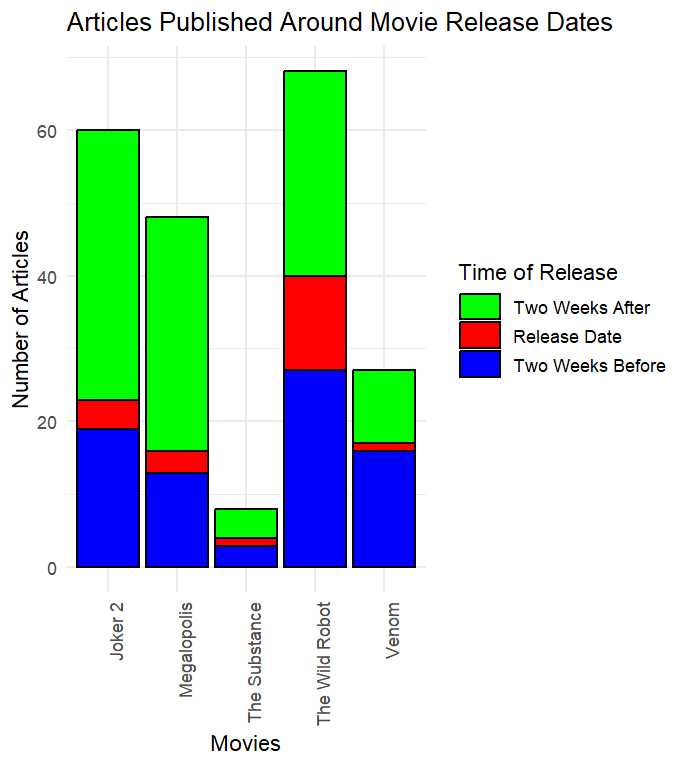
\includegraphics[width=0.4\textwidth]{Plot3.png}
    \caption{Article coverage over a 4 week span of the movies release. Note that for this plot Unrelated articles were removed to portray relevant coverage.}
    \label{fig:example-plot2}
\end{figure}

\begin{figure}
    \centering
    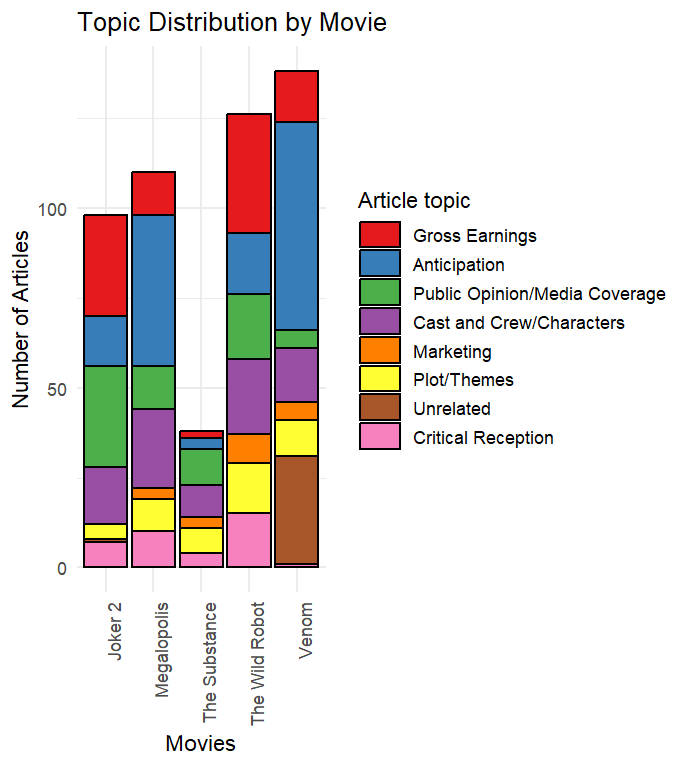
\includegraphics[width=0.5\textwidth]{Plot4.png}
    \caption{Topic distribution for each movie. Note that Venom has a significant amount of Unrelated articles.}
    \label{fig:example-plot3}
\end{figure}

\newpage 

\section{Discussion}

Regarding the total distribution of articles between the movies, we we observe that \textit{The Substance} stands out with significantly fewer articles than the others, accounting for just 7.5\% of the total. As for \textit{Joker: Folie à Deux}, \textit{Megalopolis}, \textit{Venom: The Last Dance} and \textit{The Wild Robot} account for 19.2\%, 21.6\%, 27.1\% and 24.7\% of articles respectively. 
\\
\\
From these distribution, we could argue that the coverage for each movie is accurately represented. This would be the case if not for an anomaly that came across during the analysis phase. When it came to \textit{Venom: The Last Dance} a significant portion of its articles, 30 to be exact, were unrelated and this can be observed in \textbf{Fig. \ref{fig:example-plot3}}. These unrelated articles mention venomous snakes, the comics or even a cryptocurrency called VENOM, but had no relevance with the movie. This largely inflates the coverage of \textit{Venom: The Last Dance} relative to other movies and hence the reason why it was catapulted to the top in our distribution. 
\\
\\
For a more accurate distribution observe \textbf{Fig. \ref{fig:example-plot2}} where the unrelated articles were omitted and each movie was given an equal time range (4 weeks) so that the coverage could be as unbiased as possible. The notable difference from the previously raw distribution is that \textit{Venom: The Last Dance} now has significantly less coverage. Furthermore, when observing the number of articles published 2 weeks before and after each movie release, all movies except \textit{Venom: The Last Dance} experienced either an increase in post-release coverage or remained steady. \textit{Joker: Folie à Deux} and \textit{Megalopolis} saw a rise in articles following the release, with coverage increasing by 1.95 times and 2.46 times, respectively. \textit{The Wild Robot} and \textit{The Substance} maintained a similar level of attention. Finally, \textit{Venom: The Last Dance}'s coverage took a dip after its release date and experienced a decrease by 0.64 times relative to its post-release coverage. 
\\
\\
When shifting focus to thematic analysis displayed by \textbf{Fig. \ref{fig:example-plot3}}, we observe that no single topic stands out as the predominant focus for all movies. The distribution is more varied, with individual movies having standout topic representation relative to others. Analyzing topics individually for certain movies reveals distinct patterns in the type of coverage each film attracted. 
\\
\\
For instance, \textit{Megalopolis} stands out with a focus on \textit{anticipation} and discussions about the \textit{cast and crew/characters} which speaks volumes about Francis Ford Coppola's influence and reputation within the industry. This is further backed by the TF-IDF analysis which had 'coppola' as a representative word for both these topics, and even topping the list when it came to the \textit{cast and crew/characters} category. Although, \textit{Venom: The Last Dance} was at the forefront for articles related to \textit{anticipation}, with 42.0\% of its total articles falling under the topic. A trademark when it comes to Marvel movies is their small teaser following their movie credits. At the end of the movie, Knull, a popular villain in the Marvel universe, makes a post-credits cameo appearance. Additionally, 'knull' and 'spiderman' appear in top three most popular words for the \textit{anticipation} category. As a result, the movie saw a surge of articles categorized under \textit{anticipation} which were less about the movie itself and more about the broader Marvel universe. 
\\ 
\\
In contrast, \textit{The Wild Robot} flew under the radar but was a pleasant surprise for many, garnering a good number of articles regarding \textit{public opinion/media coverage} and most notably articles concerning \textit{gross earnings}, where it had the most articles for that specific category among the other four movies. This comes as no surprise, considering that the film was hailed as a potential revival for DreamWorks, bringing a fresh new wind to the studio's reputation and highlighting its ability to produce compelling movies for all ages and of course profit, which they had been lacking in regards to box office numbers with their previous films. Second to \textit{The Wild Robot} in terms of articles discussing \textit{gross earnings} we have \textit{Joker: Folie à Deux} and not for the right reasons, the movie was seen as a commercial flop and had failed to connect with fans of the original movie. The second movie with its more artistic focus had shifted away from the darker and more raw atmosphere of the first, and this discontentment is reflected in our results. The standout article topic for \textit{Joker: Folie à Deux} is \textit{public opinion/media coverage} and for the TF-IDF results for this category 'dance' comes up as the top word which allude to the many dance and musical sequences throughout the movie. 
\\ 
\\ 
As opposed to other movies, \textit{The Substance} with relatively small coverage still managed to carve out a niche following in the media thanks to a key performance by Demi Moore playing Elisabeth Sparkle and it's bizarre and experimental storytelling. The word 'elisabeth' shows up under both \textit{critical reception} and {plot/themes}, highlighting the centrality of Moore’s character to both the film’s narrative and its reception. 
\\
\\
Finally, the \textit{marketing} category accounted for only a small fraction of the articles across all movies, indicating that while promotional efforts were present, they were not a primary focus in the overall coverage.
\\ 
\\ 
The goal of this assignment was to analyze media coverage surrounding \textit{Megalopolis}. Specifically, we were tasked with comparing its coverage to four other movies and identifying which topics within the overall coverage stand out for it. In regards to the coverage relative to other movies, we've shown that it stands shoulder to shoulder with the rest of the movies. The most prevalent category for this movie was \textit{anticipation} followed by \textit{cast and crew/characters}. We believe, that our analysis have answered Lionsgate Films demands and have provided them with valuable information and insight regarding Francis Ford Coppola's \textit{Megalopolis}.



\section{Group Member Contributions}

Owen Le Sann: Data Collection and Filtering, wrote "Introduction", "Data" and  "Methods - Initial Attempts, Data Collection and Filtering". 
\\ 
\\
Lucas Loghin: Data Analysis/TF-IDF, Plots, wrote "Discussion", "Results - Analysis Results/TF-IDF Results" and "Methods - Analysis" 
\\
\\
Giannino Lombardi: Data Annotation/Typology, wrote "Abstract", "Results - Typology Definitions" and "Methods - Typology Building" 

\bibliography{aaai24}


\end{document}

